% this is a tutorial on the basics of programming.
% it uses the R language because this is used most 
% frequently in the statistics world.
% most of the advice given here is language agnostic.
% material here is based on lessons learned from 
% Think Python by Allen B Downey
% Structure and Interpretation of Computer Programs by Abelson and Sussman
% The Art of R Programming by Norman Matloff
% (upcoming/unpublished) Advanced R development: making reusable code 
%   by Hadley Wickham and the devtools dev team
%
% Gene Hunt's tutorials have also served as a model template
%   especially given that I learned the basics from him
%
% 

\documentclass{beamer}\usepackage{graphicx, color}
%% maxwidth is the original width if it is less than linewidth
%% otherwise use linewidth (to make sure the graphics do not exceed the margin)
\makeatletter
\def\maxwidth{ %
  \ifdim\Gin@nat@width>\linewidth
    \linewidth
  \else
    \Gin@nat@width
  \fi
}
\makeatother

\IfFileExists{upquote.sty}{\usepackage{upquote}}{}
\definecolor{fgcolor}{rgb}{0.2, 0.2, 0.2}
\newcommand{\hlnumber}[1]{\textcolor[rgb]{0,0,0}{#1}}%
\newcommand{\hlfunctioncall}[1]{\textcolor[rgb]{0.501960784313725,0,0.329411764705882}{\textbf{#1}}}%
\newcommand{\hlstring}[1]{\textcolor[rgb]{0.6,0.6,1}{#1}}%
\newcommand{\hlkeyword}[1]{\textcolor[rgb]{0,0,0}{\textbf{#1}}}%
\newcommand{\hlargument}[1]{\textcolor[rgb]{0.690196078431373,0.250980392156863,0.0196078431372549}{#1}}%
\newcommand{\hlcomment}[1]{\textcolor[rgb]{0.180392156862745,0.6,0.341176470588235}{#1}}%
\newcommand{\hlroxygencomment}[1]{\textcolor[rgb]{0.43921568627451,0.47843137254902,0.701960784313725}{#1}}%
\newcommand{\hlformalargs}[1]{\textcolor[rgb]{0.690196078431373,0.250980392156863,0.0196078431372549}{#1}}%
\newcommand{\hleqformalargs}[1]{\textcolor[rgb]{0.690196078431373,0.250980392156863,0.0196078431372549}{#1}}%
\newcommand{\hlassignement}[1]{\textcolor[rgb]{0,0,0}{\textbf{#1}}}%
\newcommand{\hlpackage}[1]{\textcolor[rgb]{0.588235294117647,0.709803921568627,0.145098039215686}{#1}}%
\newcommand{\hlslot}[1]{\textit{#1}}%
\newcommand{\hlsymbol}[1]{\textcolor[rgb]{0,0,0}{#1}}%
\newcommand{\hlprompt}[1]{\textcolor[rgb]{0.2,0.2,0.2}{#1}}%

\usepackage{framed}
\makeatletter
\newenvironment{kframe}{%
 \def\at@end@of@kframe{}%
 \ifinner\ifhmode%
  \def\at@end@of@kframe{\end{minipage}}%
  \begin{minipage}{\columnwidth}%
 \fi\fi%
 \def\FrameCommand##1{\hskip\@totalleftmargin \hskip-\fboxsep
 \colorbox{shadecolor}{##1}\hskip-\fboxsep
     % There is no \\@totalrightmargin, so:
     \hskip-\linewidth \hskip-\@totalleftmargin \hskip\columnwidth}%
 \MakeFramed {\advance\hsize-\width
   \@totalleftmargin\z@ \linewidth\hsize
   \@setminipage}}%
 {\par\unskip\endMakeFramed%
 \at@end@of@kframe}
\makeatother

\definecolor{shadecolor}{rgb}{.97, .97, .97}
\definecolor{messagecolor}{rgb}{0, 0, 0}
\definecolor{warningcolor}{rgb}{1, 0, 1}
\definecolor{errorcolor}{rgb}{1, 0, 0}
\newenvironment{knitrout}{}{} % an empty environment to be redefined in TeX

\usepackage{alltt}
\usepackage{graphicx, parskip, microtype, hyperref, caption}
\usepackage{amsmath, amsthm}

\frenchspacing

\usetheme{default}
\usecolortheme{orchid}




\title{Introduction to Programming: the R perspective}
\author{Peter D Smits}

\begin{document}

\begin{frame}
  \maketitle
\end{frame}

\section{Introduction}
\begin{frame}
  \frametitle{What is programming?}

  \begin{center}
    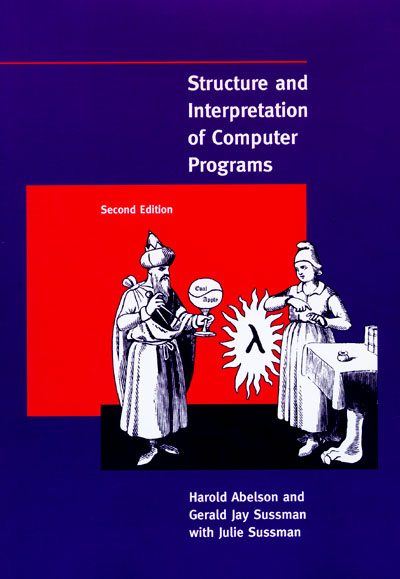
\includegraphics[height = 0.9\textheight, keepaspectratio = true]{figure/sicp}
  \end{center}

\end{frame}

\begin{frame}
  \frametitle{What is programming?}
  \textit{Structure of Interpretation of Computer Programs} by Abelson and Sussman 1996 page 1.

  \begin{quotation}
    We are about the study the idea of a \textit{computational process}. Computational processes are abstract beings that inhabit computers. As they evolve, processes maniputate other acstract things called \textit{data}. The evoution of a process is directed by a pattern of rules called a \textit{program}. People create programs to direct processes. In effect, we conjure the spirits of the computer with our spells.
  \end{quotation}

  Continued\ldots
\end{frame}

\begin{frame}
  \frametitle{What is programming?}
  \begin{quotation}
    A computation process is indeed much like a sorcerer's idea of a spirit. It cannot be seen or touched. It is not composed of matter at all. However, it is very real. It can perform intellectual work. It can answer questions. It can affect the world by disbursing money at a bank or by controlling a robot arm in a factory. The programs we use to conjure processes are like a sorcerer's spells. They are carefully composed from symbolic epressions in arcane and esoteric \textit{programming languages} that prescribe the tasks we want our process to perform.
  \end{quotation}
\end{frame}

\begin{frame}
  \frametitle{R: a brief history}
  R is a programming language based on the S language.

  Originally written by Ross Ihaka and Robert Gentleman, now by a team.

  \begin{figure}[h]
    \captionsetup{justification = raggedleft, slc = off}
    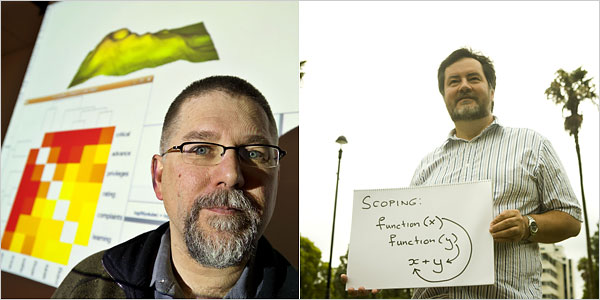
\includegraphics[width = \textwidth, keepaspectratio = true]{figure/ihaka_gentleman}
    \caption*{NyTimes}
    \label{fig:creators}
  \end{figure}

\end{frame}

\begin{frame}
  \frametitle{R: a brief history}
  Existed in a usable form since approximately 1997.

  R is kind of a messy language and pretty slow. Lots of other problems/concerns.

  Main advantages of R for statistical analysis
  \begin{itemize}
    \item designed with data in mind
    \item huge package universe
    \item lots of online resources
    \item graphics
    \item dynamic documents
  \end{itemize}

\end{frame}

\begin{frame}
  \frametitle{Console and scripts}
  The console (or REPL) is the R command line. It is the blinking cursor you stare at when you first open R. It is useful for testing bits of code and hunting for bugs in your code.

  Script files are text times with a series of commands/expessions in a row. These are then run to perform analysis. Scripts allow you to edit code and save it for later use. Write scripts, don't just use the console.

\end{frame}

\begin{frame}
  \frametitle{RStudio}
  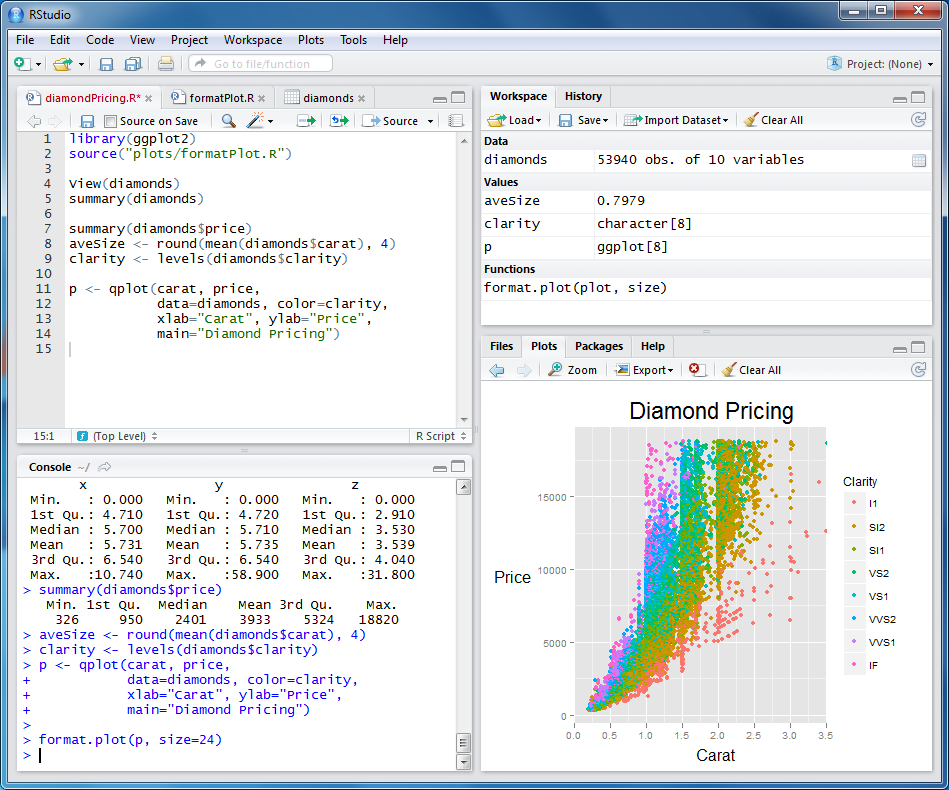
\includegraphics[height = 0.8\textheight, keepaspectratio = true]{figure/rstudio}
  % at this point it is appropriate to open up RStudio and demonstrate things

\end{frame}

\section{Programming}
\begin{frame}
  \frametitle{Using the console or REPL}

\end{frame}

\begin{frame}[fragile]
  \frametitle{Writing our first script}
  Write the following code in a script file.




\end{frame}

\begin{frame}
  \frametitle{Flow control}
  Flow control is how you tell the computer what order to do things in.

  Use TRUE/FALSE (Boolean) statements.

\end{frame}

\begin{frame}[fragile]
  \frametitle{Basics of conditional statements}
  Think about what these statements will do then try then in the console.

\begin{knitrout}\small
\definecolor{shadecolor}{rgb}{0.969, 0.969, 0.969}\color{fgcolor}\begin{kframe}
\begin{alltt}
TRUE == TRUE

TRUE == FALSE

FALSE != TRUE

2 > 1

2 < 1

\hlfunctioncall{is.numeric}(1)

\end{alltt}
\end{kframe}
\end{knitrout}


\end{frame}

\begin{frame}[fragile]
  \frametitle{\tt{if} statements}
\begin{knitrout}\small
\definecolor{shadecolor}{rgb}{0.969, 0.969, 0.969}\color{fgcolor}\begin{kframe}
\begin{alltt}
\hlfunctioncall{if}(x = TRUE) \{
  \hlfunctioncall{print}(x)
\}

\hlfunctioncall{if}(x = TRUE) \{
  \hlfunctioncall{print}(\hlstring{'yay'})
\} else \{
  \hlfunctioncall{print}(\hlstring{'boo'})
\}

\hlfunctioncall{if}(x = TRUE) \{
  \hlfunctioncall{print}(\hlstring{'yay'})
\} else \hlfunctioncall{if}(x = FALSE) \{
  \hlfunctioncall{print}(\hlstring{'what?'})
\} else \{
  \hlfunctioncall{print}(\hlstring{'why?'})
\}

\end{alltt}
\end{kframe}
\end{knitrout}


\end{frame}

\begin{frame}[fragile]
  \frametitle{\tt{while} statements}
\begin{knitrout}\small
\definecolor{shadecolor}{rgb}{0.969, 0.969, 0.969}\color{fgcolor}\begin{kframe}
\begin{alltt}
\hlfunctioncall{while} (y < 100) \{
    y <- y + 1
\}

\hlfunctioncall{while} (y < 100) \{
    \hlfunctioncall{if} (y < 0) \{
        break
    \}
    y <- y + 1
\}
\end{alltt}
\end{kframe}
\end{knitrout}


  CAUTION: \tt{while} loops can be infinite\dots

\end{frame}

\begin{frame}[fragile]
  \frametitle{\tt{for} statements}
\begin{knitrout}\small
\definecolor{shadecolor}{rgb}{0.969, 0.969, 0.969}\color{fgcolor}\begin{kframe}
\begin{alltt}
\hlcomment{# i write these a little weird so they are clearer and}
\hlcomment{# safer}

\hlfunctioncall{for} (ii in \hlfunctioncall{seq}(10)) \{
    \hlfunctioncall{print}(ii)
\}

\end{alltt}
\end{kframe}
\end{knitrout}


\end{frame}

\begin{frame}
  \frametitle{Writing our first function}
  Using what we know now, let's write our own useful function.

  Let's duplicate the sum function.

\end{frame}

\begin{frame}[fragile]
  \frametitle{Writing our first function}

  First, let's find out what sum does.

\begin{knitrout}\small
\definecolor{shadecolor}{rgb}{0.969, 0.969, 0.969}\color{fgcolor}\begin{kframe}
\begin{alltt}
x <- \hlfunctioncall{seq}(5)
\hlfunctioncall{sum}(x)
\end{alltt}
\begin{verbatim}
## [1] 15
\end{verbatim}
\begin{alltt}

y <- \hlfunctioncall{c}(1, 1)
\hlfunctioncall{sum}(y)
\end{alltt}
\begin{verbatim}
## [1] 2
\end{verbatim}
\end{kframe}
\end{knitrout}


\end{frame}

\begin{frame}[fragile]
  \frametitle{Writing our first function}

\begin{knitrout}\small
\definecolor{shadecolor}{rgb}{0.969, 0.969, 0.969}\color{fgcolor}\begin{kframe}
\begin{alltt}
sum.prime <- \hlfunctioncall{function}(x) \{
  y <- 0  \hlcomment{# storage}

\hlcomment{  # add every value of x to y}
  \hlfunctioncall{for}(i in \hlfunctioncall{seq}(\hlfunctioncall{length}(x))) \{  
\hlcomment{    # seq is for making sequences }
\hlcomment{    # length determines how long a vector is}
    
    y <- y + x[i]
  \}

\hlcomment{  # return determines the output of a function}
  \hlfunctioncall{return}(y)
\}
\end{alltt}
\end{kframe}
\end{knitrout}


\end{frame}

\end{document}
